\documentclass[12pt]{article}

\usepackage[utf8]{inputenc}
\usepackage[T1]{fontenc}
\usepackage[polish,provide=*]{babel}
\usepackage{lmodern}
\usepackage{amsmath}
\usepackage{latexsym,amsfonts,amssymb,amsthm,amsmath}
\usepackage{enumitem}
\usepackage{hyperref}
\usepackage{graphicx}
\usepackage{float}
\usepackage{subcaption}
\usepackage{booktabs}
\graphicspath{{./images/}}

\setlength{\parindent}{0in}
\setlength{\oddsidemargin}{0in}
\setlength{\textwidth}{6.5in}
\setlength{\textheight}{8.8in}
\setlength{\topmargin}{0in}
\setlength{\headheight}{18pt}

\title{Wyznaczanie ruchliwości i koncentracji nośników w półprzewodniku}
\author{Kacper Kłos}

\begin{document}

\maketitle
W poniższym artykule wyznaczyliśmy liczne parametry próbki domieszkowanego Ge o znanej geometrii. Wpierw mierząc napięcie i natężenie dostarczane na próbce, dopasowaliśmy krzywą aby określić jej przewodność w warunkach pokojowych wyznaczoną dla nas na $\sigma = 56{,}10 \pm 0{,}05 \, \Omega^{-1}m^{-1}$. Następnie wykonując pomiary dla kilku wartości natężenia i pola magnetycznego otrzymaliśmy wartość stałej hall równy $R_h = 5{,}30\times 10^{-3} \pm 0{,}03\times 10^{-3} \, m^3 C^{-1}$. Analizując dana dla pojedyńczyego pomiaru udało nam się określić znak nośników na dodatni. Łącząc poprzednie pomiary określiliśmy mobilność ładunków na $\mu = 2922 \pm 4 \, cm^2s^{-1}V^{-1}$ oraz koncentracje nośników na $1{,}1985 \times 10^{15} \pm 0{,}0013 \times 10^{15} \, cm^{-3}$, obie warości w temperaturze pokojowej. Na koniec sprawdziliśmy co dzieje się z koncentracją i mobilnością przy wzroście temperatury oraz wyznaczyliśmy energię aktywacji domieieszek. Gdy temperatura rośnie mobilność nośników maleje w przeciwieństwie do ich koncentracji, dopasowując krzywą do zaleźności temperaturowych otrzymaliśmy energię aktywacji domieszek $E_{A_s} = 0{,}658 \pm 0{,}018 \, eV$.

\newpage
\section{Wstęp}
W poniższym doświadczeniu przeprowadzimy dogłębną analizę domieszkowanej próbki Ge za pomocą amperomierza, woltomierzy, grzałki, cewek i magnetometru. Wyznaczymy przewodność próbki dla temperatury pokojowej
oraz jej stałą halla. Przy pomocy tych wartości wyznaczymy koncentrację nośników ich znak i mobilność. Na koniec zbadamy jak próbka zachowuje się w przypadku zmiennej temperatury, co dzieje się z koncentracją i mobilnością.
Na koniec dopasujemy krzywą do zależności teoretycznej dla tych zachowań i wyznaczymy energię aktywacji domieszek.

\section{Podstawy Teoretyczne}
Przedstawiona tutaj wyprowadzenie używanych w doświadczeniu wzorów jest skróconą wersją wyprowadzenia znajdującego się w \cite{skrypt}.

Podczas gdy do próbki nie jest przyłorzone żadne napięcie, nośniki ładunków poruszają się w kompletnie losowych kierunkach.
Lecz gdy na jej jednym końcu będzie większy potencjał niż na drugim wewnątrz próbki powstanie pole elektryczne.
Spowoduje ono że wciąż losowy ruch dla pojedyńczego nośnika, będzie mieć dla dużej liczby nośników, prędkość zależną od znaku nosników.
Zachowanie to możemy opisać za pomocą wzoru:
\begin{equation}
    \sigma = |q|n\mu
    \label{eq:conductivity}
\end{equation}
W którym $\sigma$ - oznacza przewodność, $q$ - ładunek każdego z nośników, $n$ - koncentracja nośników (sztuki na jednostkę objęctości), $\mu$ - mobilność nośników.

Następnie możemy rozpisać prawo ohma dla próbki: $U=RI$ gdzie $R$ możemy wyrazić przez przewodność i geometrię próbki.
\begin{equation}
    U = \frac{1}{\sigma} \frac{l}{S} I
    \label{eq:ohm_law}
\end{equation}
Gdzie $l$ - długość próbki, $S$ - pole przekroju próbki, $I$ - natężenie na próbce. Wzór ten pozwoli wyznaczyć nam $\sigma$ przez mierzalne wartości.

Finalnie kluczowe jest zrozumienie efektu Halla. Gdy przez próbke przechodzi pole magnetyczne $B$, w próbce pojawiają się dwie siły, 
jedna wynikająca z pola magnetycznego oraz druga wynikająca z ładunków osadzonych na końcu próbki przez pole magnetyczne.
\[
    F_M = q(\vec{v} \times \vec{B}), \quad F_E = U_H w
\]
Wiemy że siły po chwili zaczynają się równoważyć, co wraz z rozpisaniem $v$ pozwala nam otrzymać relację:
\begin{equation}
    U_H = \frac{1}{nq}\frac{IB}{h}
    \label{eq:hall_voltage}
\end{equation}
Współczynnik $R_H = \frac{1}{nq}$ nazywamy stałą halla. Znak napięcia halla $U_H$ pozwoli nam określić nośnik ładunków w badanej próbce.

Dla półprzewodników domieszkowanych możemy wyróżnić trzy główne zakresy zależności przewodności od temperatury \cite{skrypt}:

Zakres niskich temperatur - do około $100 \ K$, dla którego zależność opisujemy wzorem:
\[
    \sigma = \sigma_0 \exp{(-\frac{E_{A_d}}{2kT})}
\]
W którym $E_{A_d}$ jest energią aktywacji domieszek.

Zakres średnich temperatur - pomiędzy $100 \ K$ a $400 \ K$, dla którego mamy relację:
\[
    \sigma = \sigma_0 T^{-\frac{3}{2}}
\]

Oraz zakres temperatur wysokich - powyżej $400 \ K$, gdzie relacja wyrażana jest wzorem:
\begin{equation}
    \sigma = \sigma_0 \exp{(-\frac{E_{A_s}}{2kT})}
    \label{eq:high_temp}
\end{equation}
Gdzie $E_{A_s}$ jest energią aktywacji nośników samoistnych.

\section{Układ Doświadczalny}

Na diagramie \ref{fig:diagram} przedstawiony jest schemat układu elektrycznego który będziemy stosować.
Napięcia $V1$, $V2$ oraz $V3$ kontrolujemy za pomocą generatora DP832. 
Pozwala nam to zwiększać natężenia na elektromagnesie co skutkuje w mocniejszym polu magnetycznym, a także napięcie na próbce.
Wraz z układem będziemy używać magnetometru i kompasu do zidentyfikowania pola magnetycznego przez próbkę.

\begin{figure}[H]
    \centering
    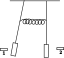
\includegraphics[scale=0.3]{diagram}
    \caption{Diagram układu pomiarowego używanego w pomiarach \cite{diagram}}
    \label{fig:diagram}
\end{figure}

Wpierw dopasujemy prostą do zależności napięcia od natężenia na próbce w celu otrzymania przewodności.

Potem wykonamy dwie serie pomiarów napięcia halla, jedna ze stałym polem magnetycznym a następna ze stałym natężeniem na próbce.
W celu zniwelowania napięć wynikających z niejednorodności próbki będziemy rejestrować napięcia halla dla czterech ustawień układu.
$U_1$ - przedstawione na diagramie $(+I, +B)$, $U_2$ - przestawiony przełącznik magnesu $(+I, -B)$, $U_3$ - przestawiony przełącznik próbki $(-I, +B)$, $U_4$ - przestawione przełączniki magnesu i próbki $(-I, -B)$.
Finalne napięcie halla wyznaczymy wzorem:
\begin{equation}
    U_H = \frac{U_1 - U_2 + U_3 - U_4}{4}
    \label{eq:effective_hall}
\end{equation}

Finalnie wybierzemy stałe napięcie na próbce i pole magnetyczne przy czym będziemy manipulować temperaturą próbki.
W tych pomiarach będzimy rejestrować spadek napięcia na próbce, temperature oraz napięcie halla.

\section{Wyniki Pomierów}
Próbka którą badamy ma wymiary $20 \times 10 \times 1 \ mm^3$ z czego będziemy korzystać w dalszej analizie.
W dalszej analizie będziemy korzystać z notacji $u(x)$ oznaczającej błąd zmiennej $x$.
A tekże wzoru na propagację błędu:
\[
    u(f(x)) = \sqrt{\sum_{i=1}^{n} (\frac{df(x_i)}{dx_i} \ u(x_i))^2}
\]

\subsection{Przewodności}
Badają zależność napięcia od natężenia dla różnych napięć dostarczanych przez zasilacz za błąd pomiarowy\cite{multimeter_hand} $u(U) = 0.5\%$ oraz $u(A) = 2\%$. 
\begin{table}[h]
    \centering
    \begin{tabular}{c|cc|cc}
        \toprule
        Nr & $I \ [mA]$ & $u(I) \ [mA]$ & $U \ [V]$ & $u(U) \ [V]$ \\
        \midrule
        1 & -26{,}82 & 0{,}1341  & -0{,}955 & 0{,}0191  \\
        2 & -20{,}08 & 0{,}1004  & -0{,}714 & 0{,}01428 \\
        3 & -24{,}74 & 0{,}1237  & -0{,}882 & 0{,}01764 \\
        4 & -19{,}73 & 0{,}09865 & -0{,}704 & 0{,}01408 \\
        5 & -9{,}69  & 0{,}04845 & -0{,}345 & 0{,}0069  \\
        6 & -4{,}70  & 0{,}0235  & -0{,}167 & 0{,}00334 \\
        \bottomrule
    \end{tabular}
    \caption{Pomiary napięcia na próbce przy zmienianym natężeniu.}
    \label{tab:ohm_measurements}
\end{table}
Do danych dopasowujemy krzywą.
\begin{figure}[H]
    \centering
    \includegraphics[scale=0.5]{ohm_law}
    \caption{Punkty pomiarowe napięcia od natężenia wraz z dopasowaniem liniowym}
    \label{fig:ohm_measurments}
\end{figure}
Z dopasowania krzywej do wartości z \ref{tab:ohm_measurements} otrzymujemy krzywą na wykresie \ref{fig:ohm_measurments} i wartości:
\begin{equation}
    R = 35{,}65 \ \Omega, \quad  u(R) = 0{,}04 \ \Omega
    \label{eq:resistance}
\end{equation}
Korzystając z równania \ref{eq:ohm_law}, wartości \ref{eq:resistance}, oraz wymiarów próbki otrzymujemy:
\begin{equation}
    \sigma = 56{,}10 \ \Omega^{-1}m^{-1}, \quad u(\sigma) = 0{,}05 \ \Omega^{-1}m^{-1}
    \label{eq:final_conductivity}
\end{equation}
Gdzie $u(\sigma)$ otrzymujemy z propagacji błędu:
\[
    u(\sigma) = |\frac{l}{whR^2} \, u(R)|
\]

\subsection{Stała Halla}
Do analizy wykorzystamy błąd pomiaroy pola magnetycznego\cite{magnetometer} $u(B) = 5\%$ oraz błąd pomiaru napięcia halla \cite{multimeter_big} $u(U_H) = 0.015\%+0{,}008\,mV$.

Zaczynając od stałego natężenia $I = -26{,}8 \ mA$ z błędem $u(I) = 0{,}6 \ mA$.
\begin{table}[H]
    \centering
    \begin{tabular}{c|ccc|ccccc}
        \toprule
        Nr & $B_+$ [mT] & $B_-$ [mT] & $u(B)$ [mT] & $U_1$ [mV] & $U_2$ [mV] & $U_3$ [mV] & $U_4$ [mV] & $u(U)$ [mV] \\
        \midrule
        1 & 53{,}3 & 56{,}8 & 2{,}84  & -7{,}44 & 8{,}13 & 7{,}43 & -8{,}15 & 0{,}01 \\
        2 & 46{,}3 & 49{,}3 & 2{,}465 & -6{,}457 & 7{,}123 & 6{,}454 & -7{,}145 & 0{,}009 \\
        3 & 38{,}8 & 42{,}5 & 2{,}125 & -5{,}430 & 6{,}159 & 5{,}424 & -6{,}148 & 0{,}009 \\
        4 & 32{,}5 & 35{,}3 & 1{,}765 & -4{,}625 & 5{,}158 & 4{,}520 & -5{,}161 & 0{,}009 \\
        5 & 18{,}5 & 22{,}0 & 1{,}1   & -2{,}572 & 3{,}245 & 2{,}560 & -3{,}256 & 0{,}009 \\
        6 & 6{,}7  & 7{,}5  & 0{,}375 & -0{,}800 & 1{,}183 & 0{,}785 & -1{,}196 & 0{,}009 \\
        7 & 63{,}8 & 67{,}4 & 3{,}37  & -8{,}80 & 9{,}54 & 8{,}79 & -9{,}57 & 0{,}01 \\
        8 & 57{,}5 & 60{,}5 & 3{,}025 & -7{,}99 & 8{,}67 & 7{,}98 & -8{,}69 & 0{,}01 \\
        \bottomrule
    \end{tabular}
    \caption{Zależność napięcia halla od iloczynu pola magnetycznego i natężenia przy stałym natężeniu}
    \label{tab:const_current_measurements}
\end{table}
Widzimy że pole magnetyczne różni się znacznie między pomiarami dlatego jako wartość używaną we wzorach będziemy brać średnią z obu. Za błąd pola uznajemy $u(B) = max(u(B_+), u(B_-))$, i taki też będziemy uznawać dla wspomnianej średniej.
Błąd pomierowy napięcia halla widniejący w tabeli to maksymalny zarejestrowany błąd napięcia.
Dopasowując krzywą za pomocą danych z tabeli \ref{tab:const_current_measurements} do wzoru \ref{eq:hall_voltage} w którym użyliśmy wzoru \ref{eq:effective_hall}, otrzyumujemy wykres \ref{fig:const_current_measuremnts}.
\begin{figure}[H]
    \centering
    \includegraphics[scale=0.5]{const_current}
    \caption{wykres zależności napięcia halla od iloczynu pola magnetycznego i natężenia przy stałym natężeniu}
    \label{fig:const_current_measuremnts}
\end{figure}
Oraz wartości:
\[
    \frac{|R_{H_C}|}{h} = 5{,}30 \ m^2C^{-1} \quad, u(\frac{|R_{H_C}|}{h}) = 0{,}03 \ m^2C^{-1}  
\]
Mnożąc przez $h$ mamy:
\begin{equation}
    |R_{H_C}| = 5{,}30\times 10^{-3} \ m^3C^{-1} \quad, u(|R_{H_C}|) = 0{,}03\times 10^{-3} \ m^3C^{-1}  
    \label{eq:hall_constant_current}
\end{equation}
Rozwarzanie znaku $R_H$ pozostawimy na później.

Analogicznie działamy dla pomiarów ze stałym polem równym $B_- = 67{,}4 \ mT$ oraz $B_+ = 63{,}8 \ mT$, biorąc średnią i rozważając błąd jak uprzednio otrzymujemy $B = 65{,}6 \ mT$ z błędem $u(B) = 4 \ mT$
\begin{table}[H]
    \centering
    \begin{tabular}{c|cc|ccccc}
        \toprule
        Nr & $I \ [mA]$ & $u(I) \ [mA]$ & $U_1 \ [mV]$ & $U_2 \ [mV]$ & $U_3 \ [mV]$ & $U_4 \ [mV]$ & $u(U) \ [mV]$ \\
        \midrule
        1 & -26{,}8 & 0{,}6 & -8{,}82 & 9{,}55 & 8{,}80 & -9{,}56 & 0{,}01 \\
        2 & -21{,}7 & 0{,}5 & -7{,}13 & 7{,}72 & 7{,}14 & -7{,}74 & 0{,}01 \\
        3 & -16{,}8 & 0{,}4 & -5{,}517 & 5{,}952 & 5{,}512 & -5{,}963 & 0{,}009 \\
        4 & -11{,}8 & 0{,}3 & -3{,}882 & 4{,}188 & 3{,}881 & -4{,}192 & 0{,}009 \\
        5 & -6{,}82  & 0{,}14 & -2{,}247 & 2{,}419 & 2{,}242 & -2{,}426 & 0{,}009 \\
        6 & -28{,}9 & 0{,}6 & -9{,}53 & 10{,}28 & 9{,}51 & -10{,}29 & 0{,}01 \\
        7 & -2{,}70  & 0{,}06 & -0{,}898 & 0{,}968 & 0{,}899 & -0{,}972 & 0{,}009 \\
        \bottomrule
    \end{tabular}
    \caption{Zależność napięcia halla od iloczynu pola magnetycznego i natężenia przy stałym polu magnetycznym}
    \label{tab:const_magnetic_field_measurements}
\end{table}
W przeciwieństwie do pomiarów ze zmiennym polem, zmienne natężenie praktycznie nie zmienia się zależnie od kierunku dlatego rejestrowaliśmy tylko jedną wartość.
Ponownie dopasowując krzywą do pomiarów \ref{tab:const_magnetic_field_measurements} do wzoru \ref{eq:hall_voltage} dostajemy wykres \ref{fig:const_field_measuremnts}: 
\begin{figure}[H]
    \centering
    \includegraphics[scale=0.5]{const_field}
    \caption{Wykres zależności napięcia halla od iloczynu pola magnetycznego i natężenia przy stałym polu magnetycznym}
    \label{fig:const_field_measuremnts}
\end{figure}
Wraz z wartościami:
\[
    \frac{|R_{H_B}|}{h} = 5{,}204 \ m^2C^{-1} \quad, u(\frac{|R_{H_B}|}{h}) = 0{,}006 \ m^2C^{-1}  
\]
\begin{equation}
    |R_{H_B}| = 5{,}204 \cdot10^{-3} \ m^3C^{-1} \quad, u(|R_{H_B}|) = 0{,}006 \cdot10^{-3} \ m^3C^{-1}  
    \label{eq:hall_constant_field}
\end{equation}
Przyczyną tego że błąd obserwowany przy pomiarach ze stałym polem jest dwa razy mniejszy od wyznaczonego dla stałego natężenia, 
jest fakt w przypadku stałego natężenia mamy punkty pomiarowe są bardziej skupione przy najniższych wartościach iloszynu $BI$ przy których błąd jest większy.


Żeby otrzymać finalną wartość $R_H$ z wartości $R_{H_C}$ oraz $R_{H_B}$ skorzystamy ze średniej ważonej wyrażonej jako:
\[
    R_H = \frac{\frac{R_{H_C}}{u^2(R_{H_C})}+\frac{R_{H_B}}{u^2(R_{H_B})}}{\frac{1}{u^2(R_{H_C})}+\frac{1}{u^2(R_{H_B})}}, \quad u(R_H) = \frac{1}{\sqrt{\frac{1}{u^2(R_{H_C})}+\frac{1}{u^2(R_{H_B})}}}
\]
Korzystając z wyznaczonych \ref{eq:hall_constant_current}\ref{eq:hall_constant_current} pozwala nam uzyskać wartości:
\begin{equation} 
    |R_H| = 5{,}208 \cdot10^{-3} \ m^3C^{-1} \quad, u(|R_H|) = 0{,}006 \cdot10^{-3} \ m^3C^{-1}  
    \label{eq:hall_const}
\end{equation}


\subsection{Znak nośników napięcia, mobilność i koncentracja ładunków}
Żeby wyznaczyć znak stałej halla przyjrzyjmy się pomiarą wykonanym równolegle z pomiarem $U_1$ w serii ze stałym natężeniem \ref{tab:const_current_measurements} i ostatnim pomiarem $U_s$ w serii \ref{tab:ohm_measurements}. 
Za pomocą kompasu wyznaczamy kierunek pola magnetycznego, które dla tych pomiarów jest skierowane z ekranu.
Widzimy że oba napięcia są negatywne, oznacza to że na rysunku \ref{fig:diagram} wyższe napięcie jest na wyjściu 5 niż na 6, oraz na wyjściu 4 niż na 3 próbki Ge.
Załóżmy że nośniki natężenia mają ładunek pozytywny, zatem będą się one poruszać od większego do mniejszego potencjału $5 \rightarrow 6$. 
Korzystając ze wzoru $F=q(\vec{v}\times\vec{B})$ widzimy że ładunki będą się zbierać przy wyjściu numer 4 tworząc tam wyższy potencjał.
Jest to w zgodności z naszymi obserwacjami, także możemy wnioskować iż nośnikami są ładunki o znaku pozytywnym czyli mamy do czynienia z domieszkowaniem p oznaczającym że wyznaczone przez nas $R_H =  5{,}208 \cdot10^{-3} \ m^3C^{-1}$.

Podstawiając do wzoru \ref{eq:conductivity} stałą halla w celu wyznaczenie mobilności nośników otrzymujemy wzory:
\[
    \mu = \sigma R_H, \quad u(\mu) = \sqrt{(\sigma u(R_H))^2+(R_H u(\sigma))^2}
\]
Który po podstawieniu naszych wyników \ref{eq:final_conductivity} i \ref{eq:hall_const} otrzymujemy:
\begin{equation}
    \mu = 2922 \ cm^2s^{-1}V^{-1}, \quad u(\mu) = 4 \ cm^2s^{-1}V^{-1}
    \label{eq:mobility}
\end{equation}
Podobnie korzystając z wartości ładunku elementarnego \cite{charge} $q=1{,}602\,176\,634 \times 10^{-19} \ C$ wraz z wartością stałej halla \ref{eq:hall_const} możemy wyznaczyć gęstość ładunków:
\[
    n = \frac{1}{R_H q}, \quad u(n) = \frac{u(R_H)}{q R_H^2}
\]
\begin{equation}
    n = 1{,}1985\times 10^{15} \ cm^{-3}, \quad u(n) = 0{,}0013\times 10^{15} \ cm^{-3}
    \label{eq:density}
\end{equation}

\subsection{Zależność temperaturowa napięcia halla}
Teraz możemy zbadać zależność napięcia halla na próbce od temperatury. W tym przypadku wykorzystamy stałe pole magnetyczne $B = 63{,}8 \ mT$ z błędem $u(B) = 4 \ mT$ oraz natężenie na próbce wynoszące $I = -26{,}9 \ mA$ przy błędzie $u(I) = 0{,}6 \ mA$.
Do mierzenia temperatury wykorzystamy termometr z błędem $0{,}1 \% + 1 \ ^{\circ}C$.

\begin{table}[H]
    \centering
    \begin{tabular}{c|cc|cc|cc}
        \toprule
        Nr & $T \ [^\circ C]$ & $u(T) \ [^\circ C]$ & $U_H \ [mV]$ & $u(U_H) \ [mV]$ & $U_P \ [V]$ & $u(U_P) \ [V]$ \\
        \midrule
        1  & 34{,}6  & 1 & -8{,}521 & 0{,}008 & -1{,}047 & 0{,}006 \\
        2  & 45{,}2  & 1 & -8{,}130 & 0{,}008 & -1{,}126 & 0{,}006 \\
        3  & 54{,}3  & 1 & -7{,}776 & 0{,}008 & -1{,}188 & 0{,}006 \\
        4  & 65{,}1  & 1 & -7{,}190 & 0{,}008 & -1{,}253 & 0{,}007 \\
        5  & 75{,}1  & 1 & -6{,}443 & 0{,}008 & -1{,}287 & 0{,}007 \\
        6  & 85{,}2  & 1 & -5{,}488 & 0{,}008 & -1{,}265 & 0{,}007 \\
        7  & 96{,}7  & 1 & -4{,}235 & 0{,}008 & -1{,}150 & 0{,}006 \\
        8  & 104{,}8 & 1 & -3{,}424 & 0{,}007 & -1{,}017 & 0{,}005 \\
        9  & 118{,}5 & 1 & -2{,}362 & 0{,}007 & -0{,}757 & 0{,}004 \\
        10 & 126{,}7 & 1 & -1{,}873 & 0{,}007 & -0{,}623 & 0{,}004 \\
        11 & 134{,}3 & 1 & -1{,}498 & 0{,}007 & -0{,}510 & 0{,}003 \\
        12 & 140{,}6 & 1 & -1{,}187 & 0{,}007 & -0{,}435 & 0{,}003 \\
        13 & 145{,}4 & 1 & -1{,}037 & 0{,}007 & -0{,}382 & 0{,}002 \\
        \bottomrule
    \end{tabular}
    \caption{Pomiary napięcia halla i napięcia na próbce poczas grzania próbki}
    \label{tab:heating_measurements}
\end{table}
\begin{table}[H]
    \centering
    \begin{tabular}{c|cc|cc|cc}
        \toprule
        Nr & $T \ [^\circ C]$ & $u(T) \ [^\circ C]$ & $U_H \ [mV]$ & $u(U_H) \ [mV]$ & $U_P \ [V]$ & $u(U) \ [V]$ \\
        \midrule
        1  & 143{,}8 & 1 & -1{,}117 & 0{,}007 & -0{,}410 & 0{,}002 \\
        2  & 136{,}2 & 1 & -1{,}402 & 0{,}007 & -0{,}506 & 0{,}003 \\
        3  & 127{,}3 & 1 & -1{,}773 & 0{,}007 & -0{,}627 & 0{,}004 \\
        4  & 120{,}3 & 1 & -2{,}183 & 0{,}007 & -0{,}742 & 0{,}004 \\
        5  & 112{,}1 & 1 & -2{,}800 & 0{,}007 & -0{,}891 & 0{,}005 \\
        6  & 105{,}3 & 1 & -3{,}408 & 0{,}008 & -1{,}018 & 0{,}005 \\
        7  & 97{,}5  & 1 & -4{,}201 & 0{,}008 & -1{,}147 & 0{,}006 \\
        8  & 86{,}6  & 1 & -5{,}452 & 0{,}008 & -1{,}258 & 0{,}007 \\
        9  & 75{,}3  & 1 & -6{,}505 & 0{,}008 & -1{,}281 & 0{,}007 \\
        10 & 66{,}2  & 1 & -7{,}219 & 0{,}008 & -1{,}255 & 0{,}007 \\
        11 & 55{,}5  & 1 & -7{,}825 & 0{,}008 & -1{,}159 & 0{,}006 \\
        12 & 44{,}2  & 1 & -8{,}267 & 0{,}008 & -1{,}112 & 0{,}006 \\
        13 & 36{,}2  & 1 & -8{,}504 & 0{,}008 & -1{,}056 & 0{,}006 \\
        \bottomrule
    \end{tabular}
    \caption{Pomiary napięcia halla i napięcia na próbce poczas chłodzenia próbki}
    \label{tab:cooling_measurements}
\end{table}

O zachodaniu badanego półprzewodnika możemy się dużo dowiedzieć przy badaniu gęstości ładunków oraz ich mobilności.
Mobilność otrzymujemy z przekształceń wzorów \ref{eq:conductivity}, \ref{eq:ohm_law} oraz \ref{eq:hall_voltage} z których otrzymamy:
\[
    \mu = \frac{U_H}{UB}\frac{l}{w}
\]
\begin{figure}
    \centering
    \includegraphics[scale=0.5]{temp_mobility}
    \label{fig:temp_mobility}
    \caption{Zależność mobilności nośników wewnątrz badanej próbki od temperatury.}
\end{figure}

Podczas gdy wzór na koncentrację ładunków wynosi:
\[
    n = \frac{IB}{hqU_H}
\]
\begin{figure}
    \centering
    \includegraphics[scale=0.5]{temp_concentration}
    \label{fig:temp_concentration}
    \caption{Zależność gęstości ładunków wewnątrz badanej próbki od temperatury.}
\end{figure}
Na wykresiach mobilności \ref{fig:temp_mobility} oraz gęstości ładunków \ref{fig:temp_concentration} widzimy że gęstośc ładunków stale rośnie podczas gdy mobilność ładunków maleje.
Może to tłumaczyć tymczasowy spadek oporu próbki na początku zwiększania temperatury obiawiający się spadkiem wartości napięcia na próbce.
Zachowanie gęstości ładunków \ref{fig:temp_concentration} możemy tłumaczyć tym że zwiększanie temperatury powoduje że coraz więcej z ładunków ma energię termiczną na poziomię przerwy energetycznej co pozwala poruszać się tym ładunką.
Podczas gdy zachowanie mobilności \ref{fig:temp_mobility} spowodowane jest zwiększonymi wibracjami sieci krystalicznej od której odbijają się nośniki.

W celu zbadania czy zbadane przez nas punkty odpowiadają zależnością temperatórowym wspomnianym w części teoretycznej dla wysokich temperatór ze wzoru na zależność przewodności od temperatury \ref{eq:high_temp} i prawa ohma \ref{eq:ohm_law} otrzymujemy:
\begin{equation}
    \log(\sigma) = \log(\frac{lI}{SU_H}) = \log(\sigma_0)-\frac{E_{A_s}}{2k}(\frac{1}{T})
\end{equation}
Tą zależność przadstawmy na wykresie \ref{fig:temp_conductivity} logarymu z przewodności $\log(\sigma)$ jako funkcja od $T^{-1}$. 
\begin{figure}[H]
    \centering
    \includegraphics[scale=0.5]{temp_cond}
    \label{fig:temp_conductivity}
    \caption{Wykres zależności otwrotności temperatury od logarytmu przewodności}
\end{figure}
Kluczowe w wykorzystaniu wzoru na przewodność \ref{eq:high_temp} jest zamienienie mierzonych przez nas stopni celcjusza na kelviny używająć wzoru $T_K = T_C + 273{,}15$\cite{kelvins}.
Skupiając się na zakresie linowym znajdującym się po lewej stronie wykresu \ref{fig:temp_conductivity} dopasowujemy linię metodą najmniejszych kwadratów.

\begin{figure}[H]
  \centering
  \begin{subfigure}[b]{0.45\textwidth}
    \includegraphics[width=\textwidth]{temp_cooling_fit}
    \caption{Dopasowanie dla ostatnich 6 pomiarów przy chłodzeniu próbki ($T>105{,}3 \ ^{\circ}C$).}
    \label{fig:temp_cooling_fit}
  \end{subfigure}
  \hfill
  \begin{subfigure}[b]{0.45\textwidth}
    \includegraphics[width=\textwidth]{temp_heating_fit}
    \caption{Dopasowanie dla pierwszych 6 pomiarów przy ogrzewaniu próbki ($T>104{,}8 \ ^{\circ}C$).}
    \label{fig:temp_heating_fit}
  \end{subfigure}
  \caption{Dopasowanie liniowe pomiarów do funkcji $\log(\sigma)$.}
  \label{fig:temp_fits}
\end{figure}
Przy chłodzeniu dopasowanie wynosi:
\begin{equation}
    \frac{E_{{A_s}_c}}{2k} = 3760 \ ^{\circ}C, \quad u(\frac{E_{{A_s}_c}}{2k}) = 150 \ ^{\circ}C
    \label{eq:temp_cooling_fit}
\end{equation}
A dla ogrzewania:
\begin{equation}
    \frac{E_{{A_s}_h}}{2k} = 3870 \ ^{\circ}C, \quad u(\frac{E_{{A_s}_c}}{2k}) = 150 \ ^{\circ}C
    \label{eq:temp_heating_fit}
\end{equation}
Duża różnica między dokładnością grzania a chłodzenia spowodowana jest błędem ludzkim, podczas ogrzewania do próbki zostało przyłorzone zbyt duże napięcie nie pozwalające zapisać wszystkich pomiarów dokładnia w tym samym momęcie.
Podobnie jak w przypadku stałej hall finalną wartość wyznaczymy poprzez średnią ważoną z dopasowania dla chłodzenia \ref{eq:temp_cooling_fit} i grzania  \ref{eq:temp_heating_fit}:
\[
    \frac{E_{A_s}}{2k} = \frac{\frac{\frac{E_{{A_s}_h}}{2k}}{u^2(\frac{E_{{A_s}_h}}{2k})}+\frac{\frac{E_{{A_s}_c}}{2k}}{u^2(\frac{E_{{A_s}_c}}{2k})}}{\frac{1}{u^2(\frac{E_{{A_s}_h}}{2k})}+\frac{1}{u^2(\frac{E_{{A_s}_c}}{2k})}}, \quad u(\frac{E_{A_s}}{2k}) = \frac{1}{\sqrt{\frac{1}{u^2(\frac{E_{{A_s}_h}}{2k})}+\frac{1}{u^2(\frac{E_{{A_s}_c}}{2k})}}}
\]
Z tych wzorów otrzymujemy wartości:
\begin{equation}
    \frac{E_{A_s}}{2k} = 3810 \ ^{\circ}C , \quad u(\frac{E_{A_s}}{2k}) = 110 \ ^{\circ}C 
    \label{eq:final_cof}
\end{equation}
Żeby wyznaczyć energię nośników wykorzystamy stałą boltzmana \cite{boltzman} wynoszącą $k=1{,}380 \, 649 \times 10^{-23} \ JK^{-1}$, możemy wyznaczyć energię ektywacji domieszek poprzez wzór \ref{eq:final_cof}:
\begin{equation}
    E_{A_s} = 0{,}658 \ eV, \quad u(E_{A_s}) = 0{,}018 \ eV
\end{equation}
Otrzymana przez nas wartość mieści się w oczekiwanch wartościach \cite{band_gap}.

\section{Podsumowanie}
Powyższy eksperyment rozpoczeliśmy od wyznaczenia przewodności próbki Ge dla temperatury pokojowej, osiągneliśmy to dopasowując krzywą do pomiarów napięcia i natężenia na próbce \ref{tab:ohm_measurements}, 
zarazem znając jej geometrię użyliśmy wzoru na prawo ohma\ref{eq:ohm_law}. Wartości uzyskane w tej części to $\sigma = 56{,}10 \pm 0{,}05 \ \Omega^{-1}m^{-1}$.
Następnie dążyliśmy do wyznaczenia stałej halla, aby otrzymać tą wartość mierzyliśmy napięcia hall a 4 różnych konfiguracjach dla stałego natężenia na próbce \ref{tab:const_current_measurements} i stałego pola magnetycznego \ref{tab:const_magnetic_field_measurements}.
Następnie wzieliśmy średnią z pomiarów i dopasowaliśmy krzywą do wzoru \ref{eq:hall_const} dla stałego natężenia \ref{fig:const_current_measuremnts} i pola magnetycznego \ref{fig:const_field_measuremnts}. 
Finalną wartość stałej halla wyznaczyliśmy jako średnią ważoną z obu serii pomiarowych i wynosi ona $R_H = 5{,}208 \times 10^{-3} \pm 0{,}006 \times 10^{-3} \ m^3C^{-1}$.
Później analizując znaki otrzymanych wartości w naszej konfiguracji przyrządów pomiarowych, doszliśmy do wniosku iż nasza próbka Ge musi posiadać nośniki o znaku dodatnim.
Potem za pomocą tych wartości i wzorów \ref{eq:ohm_law} \ref{eq:hall_const} wyznaczyliśmy mobilność na $\mu = 2992 \pm 4 \ cm^2s^{-1}V^{-1}$ oraz gęstość ładunków na $n = 1{,}1985 \times 10^{15} \pm 0{,}0013 \times 10^{15} \ cm^3$
Zmierzając do końca, zmierzyliśmy zależność napięcia oraz napięcia halla na próbce od temperatury próbki dla jej grzania \ref{tab:heating_measurements} i chłodzenia \ref{tab:cooling_measurements}.
Zbadaliśmy zależność gęstości ładunków od temperatury \ref{fig:temp_concentration} oraz ich mobilności \ref{fig:temp_mobility}.
Finalnie dopasowaliśmy krzywą do wzoru \ref{eq:high_temp} dla wysokich temperatór w naszych pomiarach ($T > 104 \ ^\circ C$) otrzymując dwie wartości dla grzania \ref{fig:temp_heating_fit} a także chłodzenia \ref{fig:temp_cooling_fit}.
Otrzymane wartości uśredniliśmy aby wyznaczyć energię aktywacji domieszek $E_{A_s} = 0{,}658 \pm 0{,}018 \ eV$.


\newpage
\begin{thebibliography}{6}

\bibitem{skrypt}
\emph{Wyznaczanie Ruchliwości i Koncentracji Nośników w Półprzewodniku}, Uniwersytet Warszawski, Marta Borysiewicz, Aneta Drabińska.

\bibitem{diagram}
\url{https://www.kicad.org/}, KiCad.

\bibitem{multimeter_hand}
\url{https://static.eleshop.nl/mage/media/downloads/bm805_datasheet.pdf}, multimetr Brymen BM805.

\bibitem{magnetometer}
\url{https://www.manualslib.com/manual/1980910/Voltcraft-Gm-70.html?page=33#manual}, miernik pola magnetycznego Voltcraft GM-70.

\bibitem{multimeter_big}
\url{http://pracownie1.fuw.edu.pl/przyrzady/Multimetr_Rigol_DM3058_UserGuide_EN.pdf}, multimetr Rigol DM3058.

\bibitem{charge}
\url{https://physics.nist.gov/cgi-bin/cuu/Value?e}, ładunek elektronu.

\bibitem{kelvin}
\url{https://www.nist.gov/si-redefinition/kelvin-introduction}, kelviny.

\bibitem{boltzman}
\url{https://nvlpubs.nist.gov/nistpubs/SpecialPublications/NIST.SP.330-2019.pdf}, stała boltzmana.

\bibitem{band_gap}
\url{https://www.ioffe.ru/SVA/NSM/Semicond/Ge/bandstr.html}, właściwości Ge.
\end{thebibliography}

\end{document}
